% This is samplepaper.tex, a sample chapter demonstrating the
% LLNCS macro package for Springer Computer Science proceedings;
% Version 2.20 of 2017/10/04
%
\documentclass[runningheads,10pt]{llncs}
%
\usepackage{graphicx}
%\usepackage{tikz}
\usepackage{cite}
% Used for displaying a sample figure. If possible, figure files should
% be included in EPS format.
%
% If you use the hyperref package, please uncomment the following line
% to display URLs in blue roman font according to Springer's eBook style:
% \renewcommand\UrlFont{\color{blue}\rmfamily}

\begin{document}
	%
	\title{Review for CACTI: Captcha Avoidance via Client-side TEE Integration}
	%
	%\titlerunning{Abbreviated paper title}
	% If the paper title is too long for the running head, you can set
	% an abbreviated paper title here
	%
	\author{Bhanuj Gandhi\orcidID{2022201068}
		\and
		Aakash Tripathi\orcidID{2022201053}
		\and
		Jatin Sharma\orcidID{2022201023}}
	%
	\authorrunning{Bhanuj Gandhi, Aakash Tripathi, and Jatin Sharma}
	% First names are abbreviated in the running head.
	% If there are more than two authors, 'et al.' is used.
	%
	\institute{International Institute of Information Technology, Hyderabad, India}
	%
	\maketitle              % typeset the header of the contribution
	%
	\begin{abstract}
		CAPTCHA is a popular method used to prevent automated bot based attacks. It requires users to solve an easy challenge that is easy for humans but tedious to solve for a machine. However, CAPTCHAs cause inconvenience to the users and are vulnerable to machine learning based attacks which can solve the puzzles with some resources. To address these issues, CACTI was proposed as an alternative approach that uses Trusted Execution Environment (TEE) to identify the legitimate users with confidence and allow them to use the service. The authors’ proposed implementation has several weaknesses, such usage of client-side TEE, relying on browser extensions, and using server-specific lists to store sensitive data, which could be a security threat to the users. This paper realizes the potential security vulnerabilities in the proposed implementation and provide the improvements to the CACTI approach, such as using cloud-based security solutions instead of TEEs, hashing the URL to generate keys instead of using plain text, and improving the threshold determination method.
	\end{abstract}
	%
	%
	%

	\section{Paper Summary}\label{summary}

	\subsection{Motivation}

	CAPTCHAs are a widely used technique which allows to differentiate between bots/computers and humans. This is a simple technique which asks the users to pass a simple test in order to access the services. But the drawbacks of CAPTCHAs are that it may be cause of frustration for legitimate users by making them solve puzzles, and can make it difficult for people with visual / hearing impairments to access the service. There has also been much research on the privacy concerns posed by the CAPCTHAs.

	\subsection{Proposed Method}

	In the paper ‘CACTI: Captcha Avoidance via Client-side TEE Integration’, the authors have tried to present a technique which can be used to avoid CAPTCHAs. CACTI as the name of the paper suggests, is bringing up a CAPTCHA avoidance protocol. This paper also brings our attention to the Trusted Execution Environments(TEE) on client’s machine processors which are assumed to be a safe and trusted area on clients machines, where any code or data residing is assumed to be non malicious. This is a very strong assumption which is taken into account as every technique or implementation specifications mentioned in the paper are based on top of these assumptions.

	To avoid captcha, the authors suggest using rate proofs to determine the legitimacy of the user. Rate proofs are cryptographic proofs that give information regarding the rate of performing sensitive actions by the client (such as clicking mouse, scrolling down etc). Rate proofs are generated on the client-side's Trusted Execution Environment. These rate proofs are an alternative way of proving legitimacy instead of solving a CAPTCHA which can be frustrating for many users. The paper further describes the properties of TEE’s and Group signatures.

	\subsection{Approach}

	The suggested captcha avoidance protocol says that when a client $(C)$ requests access to a service on Server $(S)$, the server sends back a threshold starting time $(t_s)$, a new timestamp(t), threshold count k. If the activity of the client is below that threshold, the server won’t send CAPTCHA to the client,  the server sends a threshold starting time $(t_s)$, a new timestamp(t), threshold count  $k$,. If the activity of the client is below this threshold, then to prove it to the server, it sends back a rate proof which is generated through its TEE to the server, which will be later verified by the server. Client has to maintain server-specific lists and global-lists.

	\subsection{Design}

	The various design challenges faced revolve around TEE like its memory limitations, limited monotonic counters or its entry or exit overhead. Now, because the websites need to understand different Trusted Execution Environment(TEE) types, a separate Provisioning Authority is introduced in this paper which is responsible for TEE attestation verification. Trust between PA and TEE is assumed and if it isn’t the case, then the user falls back to solving CAPTCHA again. Client’s TEE must store all timestamps, but since this is not possible due to limited storage provided by TEE, they are stored in an outside database with the help of Hash chains of timestamps and Merkle Hash Trees for achieving data integrity.

	In order to produce rate proofs, the client provides list and timestamps information to TEE. TEE then performs the hash checks, MHT checks and also starting and updating lists. Since the client has to maintain a timestamp list, storage requirements turns out to be a concern. In order to solve this, the paper suggests list pruning such that all the timestamps before the current timestamp sent by the server are merged. It is assumed that the server sends timestamps in increasing order only as it is sending current timestamps.

	\subsection{Analysis \& Results}

	CACTI implementation is addressed in this paper by creating a browser extension(specific to Google chrome). CACTI is integrated into websites by using HTML scripts with CACTI-div elements. This paper also talks about various security concerns it brings. It talks about attacks like data integrity and rollback, timestamp omission, list substitution, TEE reset, CACTI Botnets, malware,client tracking and other DOS attacks.

	They talked about latency evaluations which were performed in four phases: Init-Enclave(where host retrieves data from database and initializes MHT within enclave),Pre-Enclave(host gets hashes and timestamps from database), In-Enclave and Post-Enclave(host updates/inserts data). On varying the number of timestamps to 10,000 in a query, the latency is only 40 ms.They also experimented with varying the number of lists, signature operation latency and end to end latency which turns out to be below 250 ms. As far as bandwidth is concerned, CACTI achieves at least 97\% reduction in client bandwidth as compared to standard reCAPTCHA solutions. Author has also talked about database and system-level optimizations at the end of the paper.



	\section{Critiques}

	\subsection{Assumptions  \label{sec1}}

	We have carefully studied the paper and assumptions that are mention, some of the assumptions that we find too strong to make are mentioned below

	\begin{enumerate}
		\item \textbf{Assumption}: Authors have assumed that the device on which the proposed method will run must have \textit{Trusted Execution Environment} (TEE) enabled. They have also assumed that the proposed approach will work on any TEE enabled device.

		\textbf{Problem}: Although Trusted Execution Environments are rapidly increasing in the devices, it is still a growing technology and not all devices are TEE enabled. As mentioned in \ref{summary}, TEE(s) are used for protection of sensitive data and processes. It is isolated from the main operating system. It is not safe to assume that all TEE enabled devices work the same way, different operating systems have different hardware architecture implementation of TEE for eg: \textit{Arm TrustZone}, \textit{iOS Secure Enclave}, \textit{Intel SGX}, etc.\ It also depends on the different system policy, it would not be possible to implement a general application that will suffice these system requirements.\\

		\textbf{Solution}: Instead of using TEE on the client machine, we can use Cloud-Based security methods that can provide similar level of security. The sensitive data processing that are proposed to happen in the TEE, can be performed on Cloud remote server as proposed by Zhou et al.\cite{ref1}. This approach involves various entities to compute a certain function jointly without exposing their private information. The client device will send a list timestamps (rate proofs) based on certain actions securely through MPC Protocol. Using the logic proposed by CACTI, we server will check the number of timestamps and match it with the threshold and returns the result to the server. Server can then check if the user is legitimate, if not the fallback CAPTCHA will be shown to the user. This approach will resolve the hardware requirements for client devices. This will eliminate the dependency on client device whether it is TEE enabled or not.\\

		\item \textbf{Critique}: In the paper, the proposed approach by the authors has assumed that the server or the website admin decides the appropriate number of threshold values (k). This value is used to determine whether the client is legitimate or a bot. Authors proposed that the server will ask for the rate-proof by the client. Server will send a timestamp ts to the client’s TEE and it will check if the intended list of timestamps has k or less number of nodes greater than the timestamp ts. TEE also verifies if the incoming timestamp (ts) is greater than the latest timestamp of the list, if both of the conditions satisfies, then TEE sends an encrypted authorized request and the server allows the client to enter the website without any CAPTCHA. Authors nowhere mentioned how to determine the value of k. In our opinion, k is the most important hyperparameter of this approach. If we take the value of k too high, then it will allow bots also to perform malicious activities, and if we take the value of k too low, then even the legitimate user has to solve the CAPTCHA to enter the website. Thus, making this approach equivalent to using CAPTCHA only.\\

		\textbf{Solution}: One possible way to determine the value of threshold is to find the expected number of requests per unit time, this can depend on various use-case. For eg. a form website might require a lot of keyboard events, a news website might require very less number of keyboard events. According to the usability statistics, traffic admin can determine the number for threshold. The value of threshold can also be learned overtime. We can use a machine learning model that learns the behaviors of the client over-time and dynamically updates the value of threshold. Taking up the dynamic approach will also add a layer of security for the proposed method as attackers will not be able to learn the value of threshold and cause the denial of service attacks. Dynamic threshold will also help systems learn the analytics of the clients and can take certain security actions using them. The end goal is still preserved that is to let legitimate user bypass the CAPTCHA whereas preventing attackers from performing Denial of Service (DoS) Attacks.\\


	\end{enumerate}

	\subsection{Technical approach  \label{sec2}}

	\begin{enumerate}
		\item \textbf{Problem:} In the paper, authors have mentioned \textit{proof-of-concept} implementation of client-side browser extension. They defined the use-case of this browser extension as follows
		There are two parts in the extension:
		\begin{enumerate}
			\item \textbf{Content Script}: This part checks the HTML page of the website and scans for div with id \textit{CACTI-id}, if it is present, a request will be forwarded to the background script.
			\item 	\textbf{Background Script:} It launches the host application in the client machine using Chrome Native Messaging API and maintains the information of the PORT the application is running throughout the browser session.
			The server keeps on sending notification to the proposed browser extension for each request, user has to provide the rate-proof by allowing through the browser extension and they also mentioned a default allow feature that will use it’s PA (Host Application) to access the TEE without asking the client.\\
		\end{enumerate}


		\textbf{Critique:} The proposed browser extension method may introduce a lot of potential hazards. Attackers can create a malicious browser extension and gain access to the client's TEE. As TEE is used for processing a lot of sensitive information and this method can cause potential damage. Paper proposed by Aurore Fass et al.\cite{ref2} describes how browser extensions can collect data from the client machine and communicate with the web APIs to share it. We understand that Chrome has its own mechanism to flag an extension safe or malicious, still there are a couple of extensions that may cause privacy issues. Using browser extensions, attackers can have access to a lot of privileged information, which can then use extension’s communication APIs to send vulnerable payloads. The communication flow of data is shown in Fig. \ref{fig:browserfig}, and attackers can add event listeners, send/receive messages through APIs easily to exploit the client’s privacy.

		\begin{figure}[h]
			\centering
			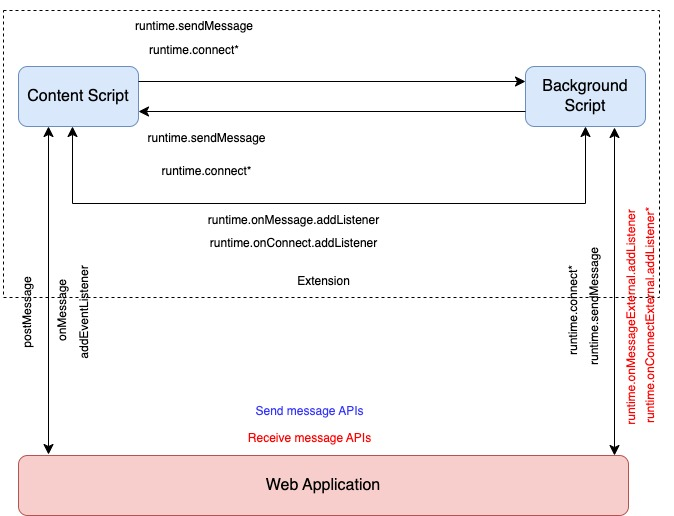
\includegraphics[scale=0.5]{./imgs/browser_extensio_flow.jpg}
			\caption{Data-flow Diagram of Browser Extension \cite{ref2}}
			\label{fig:browserfig}
		\end{figure}

		\textbf{\\Solution:} Keeping in mind the vulnerabilities of browser extensions, authors should propose a native browser based implementation, we can natively integrate the CACTI implementation functionality in the browser architecture so that no malicious user can tamper or inject their own code to perform attacks, this will eliminate the need for a separate browser extension. This approach will reduce the risk of attack and improve the security of CACTI. Only requirement to implement this is that the browser itself needs to have access to a TEE. There are several browsers that natively support secure enclaves such as Intel SGX, etc. Many browsers provide a secure sandbox environment which can achieve the same goal with enhanced security.\\

		\item \textbf{Critique}: In order to reduce client storage overhead, this paper suggests pruning the timestamp lists by merging all the timestamps before a certain time $t_P$ with just a number. They claim that the server will not ask for the rate proofs before a certain time $t_P$, this will not hamper the security of CACTI server can still get the legitimate rate proofs but it will increase the security in a manner that if any malicious user who does not know the time $t_P$ will try to access the list will always get a number greater than a threshold and they would not be able to generate rate proofs. This methodology introduces a new domain of attacks for malicious users. Attackers can act as a server and send a dummy future timestamp, then the client’s TEE won’t be able to generate \textit{‘rate of proof’} for future timestamps, thus leading to denial of service. Similarly if an attacker sends a past timestamp and if client had already pruned the timestamp list then the rate of proof generated by client would be very large which exceeds threshold and leading to denial of service again. \\

		\textbf{Solution}: For mitigating future timestamps issues, the client’s browser extension can simply check if timestamp $t_P$ is a future timestamp or not. This will prevent malicious timestamps to hit client. Whereas, for past timestamps, in order to solve the pruning issue, we can have the timestamps stored as numbers in ranges of specific time intervals. Say, we have bins of size $500ms$. So the number of timestamps between $500ms$ is stored as a simple count. This information about the storage of timestamps must be already known to the server, PA and client so that the server can ask for rate proofs in the multiple of bin size($500ms$ in the above case). Also, we can restrict the server to send timestamps until a certain time frame only, like the past 7 days or so. So that the client can keep forgetting the previous data and save storage space. If the server asks for rate proof in the previous 2 seconds, then the rate proof will be simply the sum of the last 4 bins. This way we can avoid DOS attacks with being efficient in timestamp storage and applying a few checks on the timestamps arriving.\\

		\item \textbf{Critique:} In the paper, authors have mentioned that there will be two types of list that needs to be stored in the TEE, one is the server-specific list and other would be the global list. Authors proposed that the name of the server-specific list could be the URL of the website but making the URL as a key in plain text can increase the vulnerability in the system. Any attacker who gains access to the client would easily know for which  website this specific list belongs to and can forge/taper it to cause privacy harm. This idea of storing plain text URLs makes it easier for the attacker to decode the information about the proposed security system.\\

		\textbf{Solution:} Instead of storing the URL as a plain text key, we could hash the URL before using it as a key of the server specific list. Another feasible method to improve this system is to make key robust instead of directly hashing the URL. Possible approach could be the usage of a combination of different parameters of the system. Those parameters could be a URL string with Client’s IP address or initial timestamp provided by the server. The goal is to prevent the system's security from being compromised. This method ensures that server specific lists are stored securely and can be used by the intended entities in this case server and PA (Provisioning Authority). The following suggested mechanism is shown in the Fig \ref{fig:hasfig} in which we have shown how we can store the key as a hash of URL and client’s IP.\\

		\begin{figure}[h]
			\centering
			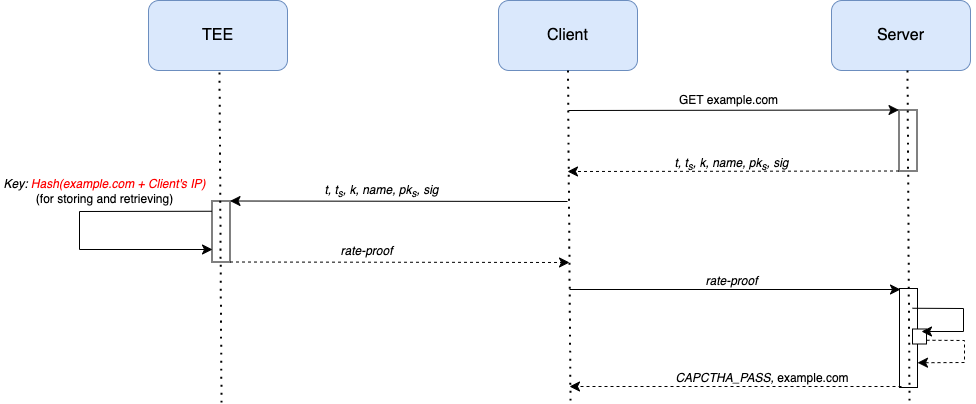
\includegraphics[scale=0.35]{./imgs/hash_diag.png}
			\caption{Improved method to store the key in TEE}
			\label{fig:hasfig}
		\end{figure}

		\item \textbf{Critique}: Authors understand that most of the TEEs have a limited amount of protected memory and limited number of counters in the implemented architecture. To resist this problem authors have mentioned the use-case of the external databases to store the protected data. Authors have mentioned the standard database and provided a method to store the timestamps data securely in the database. Fig \ref{fig:hashfig} depicts how the chain of hashes are stored in the database so that malicious users can tamper the list and integrity of the data is maintained.

		\begin{figure}[h]
			\centering
			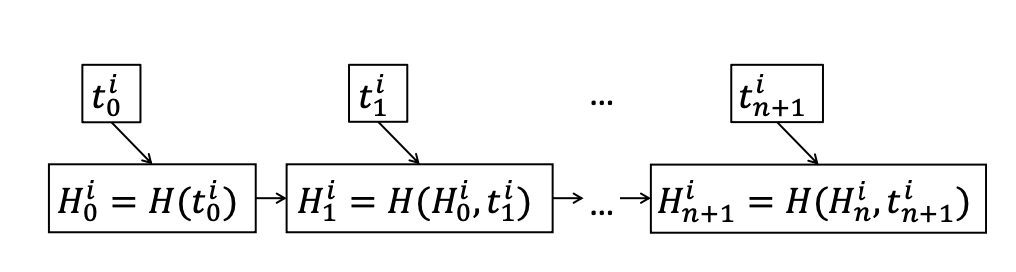
\includegraphics[scale=0.35]{./imgs/img4.png}
			\caption{Improved method to store the key in TEE \cite{ourpaper}}
			\label{fig:hashfig}
		\end{figure}

		To minimize the storage, authors have also adapted the Merkle Hash Trees (MHTs) to maintain the integrity and rollbacks. But the problem is that storing this secure data in an external database creates vulnerabilities for the system. In \cite{ref3} Mark A. Williams et al., have discussed potential vulnerabilities using the National Vulnerability Database. The study uses various machine learning models to predict the patterns in the vulnerability. They found that the number of reported vulnerabilities have been increasing with time and the internet based vulnerabilities are becoming more prominent. \cite{url1} provides various growing vulnerabilities in the databases. There are several ways that the database can be compromised.\\

		\textbf{Solution:} Instead of storing the data in the external databases, we should compress the data in some form and store it in the TEE memory itself. Statistics can be compressed using various string compression methods which will have an overload of compressing the string every time but surely increase the security of the system and can prevent several potential attacks. There are several data compression techniques proposed over the past year. DEFLATE\cite{sec5} is a lossless data compression algorithm which uses LZ77 and Huffman coding mixtures to compress the data, LZ4\cite{sec4} is another fast, lossless compression algorithm which is used in real time databases, Brotli\cite{sec2} is another lossless data compression developed by Google which is specifically optimized for web services. Zstd\cite{sec3} is very fast and has high compress ration The implementation of these methods can increase the security of the system and make it more robust.\\

		\item \textbf{Critique}: The paper introduces a provisioning authority which is responsible for verification of TEE attestation. It is assumed that there is trust and compatibility between PA and TEE. But this can lead to bypassing this CACTI\cite{ourpaper} technique if this assumption is considered false. There are very few devices which have provisioning authorities installed. Thus, to reach a state where the 3.5 billion CAPTCHA users will have PA installed that too which is compatible with their Trusted Execution Environment, seems a bit far-fetched idea. Also, the installation of compatible PA on a client's machine can be a bit of an advanced task for inexperienced users. The overall purpose of this CACTI\cite{ourpaper} is to reduce the clients efforts which are expected to vanish by introducing so many layers. Also, a malicious PA might try to hamper clients privacy as PA’s know the rate of proofs generated with the client. This sensitive information can be easily traded.\\

		\textbf{Solution}: With proper research either the concept of Provisioning Authority should be dropped or proper, secure and less complicated alternatives can be brought up with a universal design so that it can be compatible with Trusted Execution Environments.\\

		\item \textbf{Critique:} Many TEEs use some online services for remote attestation. Intel SGX uses Intel Attestation Service (IAS) to perform remote attestation. ARM TrustZone, which is used in a wide variety of devices, including smartphones, tablets, and IoT devices, uses an online attestation service called GlobalPlatform Compliance Program. Qualcomm Secure Execution Environment (QSEE), which is used in many Android smartphones and tablets, uses Qualcomm Secure Execution Environment Online Service to perform remote attestation. Microsoft Virtual Secure Mode (VSM), which is used in Windows 10 Enterprise and Windows Server 2016, uses an online attestation service called the Windows Defender System Guard. Google Titan M which is used in Google Pixel devices uses Google Cloud Titan Attestation Service.
		If the online servers are down for some reason, or the clients and the servers are part of some local area network, then these online attestation services will not be accessible. In this case, all the legitimate users will receive CAPTCHAs as the group signature generated by the TEE won’t be verifiable. \\

		\textbf{Solution}: If the online attestation services are down, a solution can be to use local attestation mechanisms to perform attestation between two enclaves without using the online attestation mechanisms. These local mechanisms are provided in Intel SGX and ARM TrustZone. However, it should be noted that offline attestation mechanisms may have limited functionality compared to the online ones and may not be suitable for all use cases. Some security requirements may mandate the use of online attestation services.

		If the online attestation services are down and the clients and servers are not part of any local network and are able to access the internet, then a possible solution can be to create redundant copies of these services and deploy them on different servers at different locations. When the primary servers are down, the redundant servers can be used.

		Another solution can be to use a pre-computed set of attestation results that were generated and securely stored ahead of time. When the servers are down, these pre-computed results can be used by the provisioning authorities to verify the integrity of the TEEs.\\

		\item \textbf{Critique} The authors introduce a concept of Provisioning Authorities. It should be the responsibility of the provisioning authorities to implement the solution mentioned in critique 2. Though the authors mention the concept of provisioning authorities, at the present time, these authorities are very limited as setting up of provisioning authorities can be complex and challenging because it requires dealing with multiple TEE vendors, establishing proper coordination and cooperation between them to make a secure and trusted infrastructure for provisioning and managing user credentials within the TEE.

		Also since different TEEs have different security mechanisms and protocols, for making a centralized provisioning authority, different TEE vendors must understand the security protocols of each other’s TEE, which may be very difficult as it may involve vendors sharing patented information about their TEE to other vendors. Even if this happens, the patented and secure protocols of TEE, knowledge of which was limited to one organization/vendor earlier, will now be known to multiple organizations/vendors which can compromise the security of TEEs.\\



		\item \textbf{Critique}: CACTI\cite{ourpaper} does the rate proof generation on clients' Trusted Execution Environment, which can be considered as an overhead because TEE is a very restrictive part of clients machines with limited memory capacity. A question arises that why should a legitimate client be using its own resources to prove its legitimacy time and again. Even though this is happening in the background, attackers can exploit client’s resources by accessing TEE.\\

		\textbf{Solution}: The generation of the rate of proof must be shifted from the client's machine. It can either happen on server by monitoring client’s action or on third party trusted services which can have better storage capacity as well as better computation facilities. Even though we might use a third party service, we must ensure that it is facilitated to the client as a service itself and the client should not have a headache of enrolling in third party services.\\

		\item \textbf{Critique:} Suppose a client tries to login into a website. To identify the legitimacy of a user, the server sends a threshold starting time ($t_{s}$), a new timestamp($t$), threshold count $k$, its private key($p_k$), its name name, and its signature($sig$). It asks the user “if there are no more than $k$ timestamp since $t_s$, store $t$ and provide a rate proof”. If the client's activity is less than $k$, it will not receive any CAPTCHA, else, it will receive a CAPTCHA on the suspicion of an illegitimate user by the server.

		The problem of this approach is that any machine that accesses the website can easily determine the value of $k$. Even if the value of $k$ is encrypted, using various machine learning algorithms, the value of $k$ can be determined (like by trying different values of k and finding the point at which the server stops sending CAPTCHA). Once the value of $k$ is determined, the bot needs to ensure that it limits its activity below $k$ while accessing that particular website. If the bot is successful, it won't receive any CAPTCHA from the server and will easily bypass the security check that is provided by CAPTCHA. It won't even have to try solving the CAPTCHA as the server never sends it thinking that the bot is a legitimate user.\\


	\end{enumerate}

	\subsection{Results \& Analysis  \label{sec3}}

	\begin{enumerate}

		\item\textbf{Critique}: The paper talks about Server load evaluations and concludes that server load in CACTI\cite{ourpaper} is less as compared to standard CAPTCHA mechanisms. In the results and analysis part authors have mentioned the metrics reached in terms of data usage, bandwidth usage, and server load. But it fails to talk about client load. As we mentioned in this review that the processing of rate proof is done on client side, the client-side load will be more than the standard CAPTCHA mechanisms. Authors have not talked about this aspect, whereas it is one of the most important aspects of this paper as it requires the client to have some TEE space reserved for CACTI\cite{ourpaper} rate proof computation and also to have some storage reserved for storing timestamp lists. Authors have also failed to mention the computation at TEE part and how much CPU usage and memory the browser extension is consuming.\\

		\textbf{Solution:} Several tests can be implemented at the client machine to check the usage of client's resources. Periodic memory checks and CPU usage will be able to tell how efficient this method is for the client. After evaluating all such metrics would be a good way to analyse the proposed method.\\

		\item \textbf{Critique}: Even after adding all these resources, layers, protocols and solutions to CACTI\cite{ourpaper}, this paper still is not able to completely replace CAPTCHA with CACTI. Many times in this paper it is mentioned that if something does not work, the fallback is always CAPTCHA and even after proving rate proofs, a client may still have to solve CAPTCHA at times.\\

		\textbf{Solution:} Although authors have mentioned that the fallback will always be the CAPTCHA, in order to make it a robust technique that can really solve the security issues in the world, there should be some other fallback method which is based on the CACTI\cite{ourpaper} as well. After having a lot of data and time-stamps from the client, there should be an algorithm to make a concrete decision for the server to decide whether it is a legitimate user or a bot who can perform a malicious activity.

	\end{enumerate}


	\subsection{Improvements}

	Based on all the above mentioned critiques in \ref{sec1}, \ref{sec2}, and \ref{sec3} below are some of the improvements that can be implemented in CACTI \cite{ourpaper} to make it more robust and less susceptible to the malicious attacks

	\begin{enumerate}
		\item We have proposed that instead of using the client-side TEE and utilize more of the system resources, cloud-based security solutions can be used such as using Secure Multiparty communication (MPC) Protocols in the cloud servers.

		\item We have also proposed a dynamic way to decide the threshold so that the intended design adapts to the threshold value and based on the behaviors of the user, the server decides with the confidence that which user is legitimate or which user is malicious.

		\item We have also proposed a browser implementation of CACTI \cite{ourpaper} which is less prone to the attacks and more secure instead of using browser extension as mentioned in the intended design. We have also proposed that instead of using TEE, browser can use secure sandbox environment to achieve the same goal with enhanced security.

		\item We have also proposed a methodology to prevent Denial of Service attacks in the system by providing alternative method to prune the timestamps which saves the space used as well as provide a more robust security.

		\item We have also proposed that to make sure attacker or malicious user does not know the value of the threshold and train its system to bypass this method, we can use machine learning model to decide the threshold value at the runtime.

		\item As the proposed design directly stores the plain URL text as a key for the list in TEE, we have proposed a method that takes a combination of URL and other client parameters as a combination and hash them to use as a key to make the system more secure. This will help in accessing the data only to the intended entities even if database is compromised.

		\item As the main module of the CACTI \cite{ourpaper} system is TEE, there are some TEEs which allows online attestation which requires internet or access to public APIs. To overcome that we have suggested to use the offline services, or the services which are highly scalable and secure in order to make the process more secure.

		\item In the proposed design, authors have mentioned the use of external databases which are prone to attacks and are vulnerable. To mitigate this issue, we have proposed a new mechanism to store the data in the limited memory by using various compression algorithm, which are fast as well as high compress ratio and store the data in TEE itself. This will increase the security of the system and make it more robust.

	\end{enumerate}

	%
	% ---- Bibliography ----
	%
	% BibTeX users should specify bibliography style 'splncs04'.
	% References will then be sorted and formatted in the correct style.
	%
	% \bibliographystyle{splncs04}
	% \bibliography{mybibliography}
	%

	\begin{thebibliography}{8}
		\bibitem{ourpaper}
		Nakatsuka, Y., \& Ozturk, E. (2021, January). CACTI: Captcha avoidance via client-side TEE integration. In 30th USENIX Security Symposium (USENIX Security 21).



		\bibitem{ref1}
		Zhou, X., Xu, Z., Wang, C., \& Gao, M. (2022, June). PPMLAC: high performance chipset architecture for secure multi-party computation. In Proceedings of the 49th Annual International Symposium on Computer Architecture (pp. 87-101).

		\bibitem{ref2}
		Fass, Aurore, et al. "Doublex: Statically detecting vulnerable data flows in browser extensions at scale." Proceedings of the 2021 ACM SIGSAC Conference on Computer and Communications Security. 2021.

		\bibitem{sec1}
		Leavline, E. J., \& Singh, D. A. A. G. (2013). Hardware implementation of LZMA data compression algorithm. International Journal of Applied Information Systems (IJAIS), 5(4), 51-56.

		\bibitem{sec2}
		Alakuijala, J., Farruggia, A., Ferragina, P., Kliuchnikov, E., Obryk, R., Szabadka, Z., \& Vandevenne, L. (2018). Brotli: A general-purpose data compressor. ACM Transactions on Information Systems (TOIS), 37(1), 1-30.

		\bibitem{sec3}
		Chen, J., Daverveldt, M., \& Al-Ars, Z. (2021, June). FPGA Acceleration of Zstd Compression Algorithm. In 2021 IEEE International Parallel and Distributed Processing Symposium Workshops (IPDPSW) (pp. 188-191). IEEE.

		\bibitem{sec4}
		Bartík, M., Ubik, S., \& Kubalik, P. (2015, December). LZ4 compression algorithm on FPGA. In 2015 IEEE International Conference on Electronics, Circuits, and Systems (ICECS) (pp. 179-182). IEEE.

		\bibitem{sec5}
		Deutsch, P. (1996). Rfc1951: Deflate compressed data format specification version 1.3.

		\bibitem{url1}
		https://www.datasunrise.com/potential-db-threats/10-common-vulnerabilities/

		\bibitem{ref3}
		Williams, M. A., Dey, S., Barranco, R. C., Naim, S. M., Hossain, M. S., \& Akbar, M. (2018, December). Analyzing evolving trends of vulnerabilities in national vulnerability database. In 2018 IEEE International Conference on Big Data (Big Data) (pp. 3011-3020). IEEE.

	\end{thebibliography}



\end{document}
